\subsection{The Fourth Refinement}
\label{sec:component_diagrams-tutorial_fourthRefinement}

 
The washing machine sub-system is now further partitioned into 2 components: the drum sub-system and an abstract component representing the remaining washing machine sub-system, following the pattern of previous refinements.
The component diagram is shown in Figure \ref{fig:FourthRefinementOfWashingMachine}.
Three boolean connectors pass messages from the washing machine sub-system to the drum to open and close the hot or cold water valves and to switch the drain pump on or off. Two further natural number connectors pass the water level and the water temperature back from the drum to the washing machine sub-system.
 
 \begin{figure}[!htbp]
  \centering
  \ifplastex
  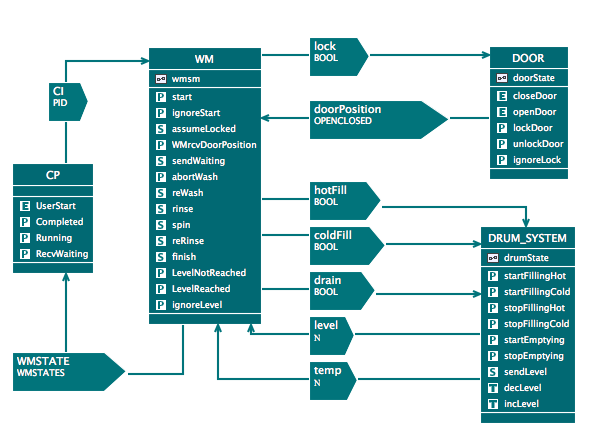
\includegraphics[width=1024]{figures/image41.png}
  \else
  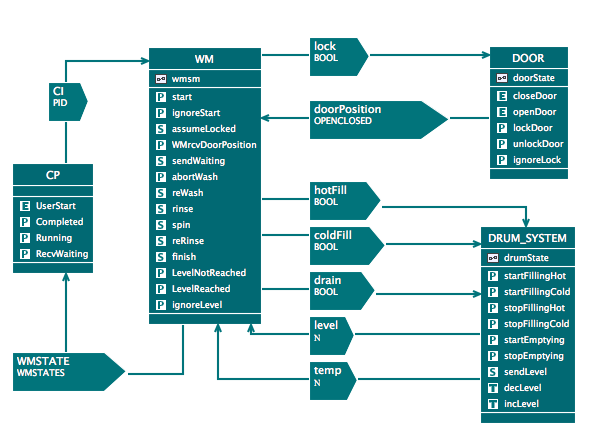
\includegraphics[width=1\textwidth]{figures/image41.png}
  \fi
  \caption{Fourth Refinement of Washing Machine}
  \label{fig:FourthRefinementOfWashingMachine}
\end{figure} 
 
The state machine for the drum sub-system is shown in Figure \ref{fig:FourthRefinementStatemachineForTheDrumComponent}.
 
 \begin{figure}[!htbp]
  \centering
  \ifplastex
  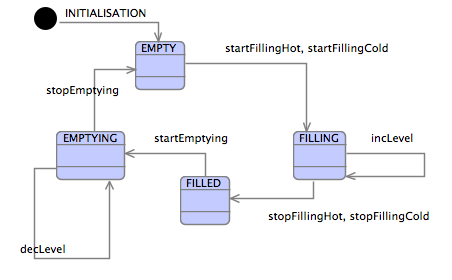
\includegraphics[width=1024]{figures/image42.png}
  \else
  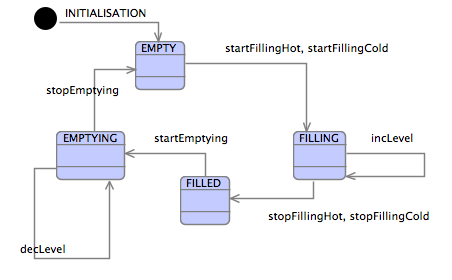
\includegraphics[width=1\textwidth]{figures/image42.png}
  \fi
  \caption{Fourth Refinement : State-machine for the Drum Component}
  \label{fig:FourthRefinementStatemachineForTheDrumComponent}
\end{figure} 
 
The washing machine state machine is now further refined to manage the filling and emptying of the drum by monitoring the water level as shown in Figure \ref{fig:FourthRefinementRefinedStatemachineOfTheWashingMachine}.
 
 \begin{figure}[!htbp]
  \centering
  \ifplastex
  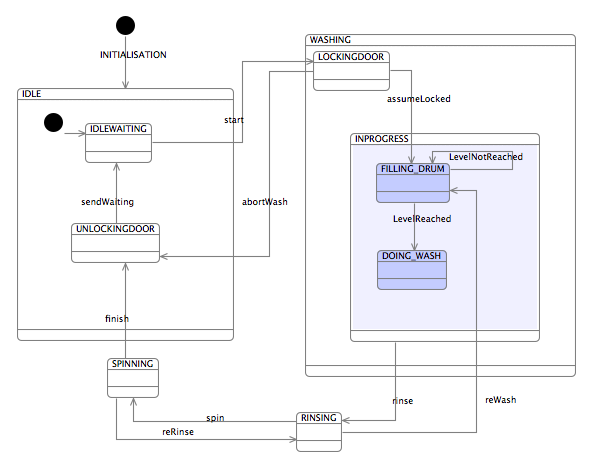
\includegraphics[width=1024]{figures/image43.png}
  \else
  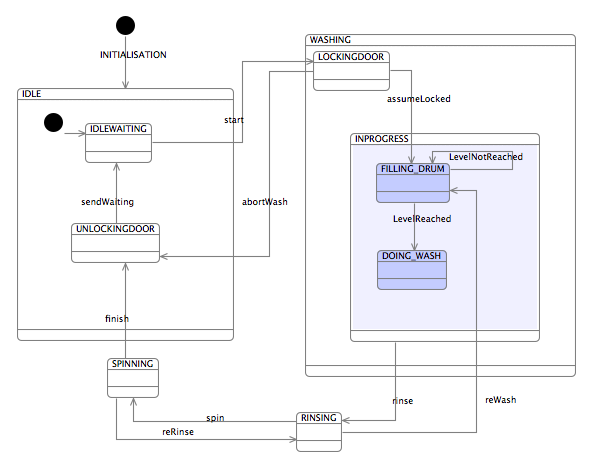
\includegraphics[width=1\textwidth]{figures/image43.png}
  \fi
  \caption{Fourth Refinement : Refined State-machine of the Washing Machine}
  \label{fig:FourthRefinementRefinedStatemachineOfTheWashingMachine}
\end{figure}  
 
The value TRUE is sent on the coldFill connector as shown in Figure \ref{fig:FourthRefinementPortSendOnTheColdFillConnector}.
 
 \begin{figure}[!htbp]
  \centering
  \ifplastex
  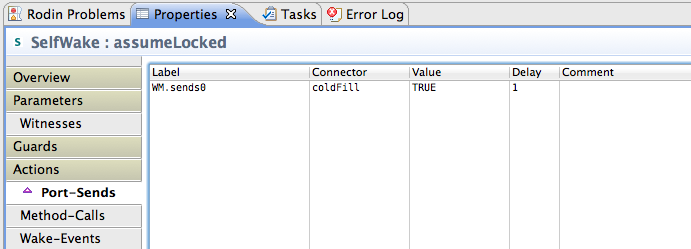
\includegraphics[width=1024]{figures/image44.png}
  \else
  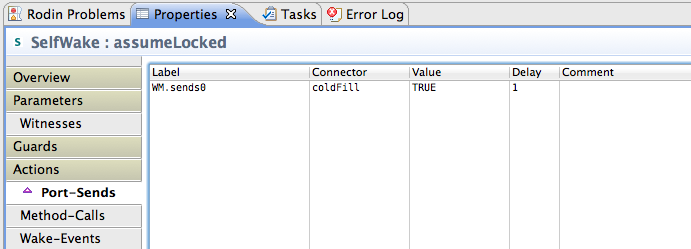
\includegraphics[width=1\textwidth]{figures/image44.png}
  \fi
  \caption{Fourth Refinement : Port Send on the coldFill Connector}
  \label{fig:FourthRefinementPortSendOnTheColdFillConnector}
\end{figure} 
 
The drum sub-system receives the value on the coldFill connector and starts filling the drum (Figure \ref{fig:FourthRefinementPortWakeOnTheColdFillConnector}).
 
 \begin{figure}[!htbp]
  \centering
  \ifplastex
  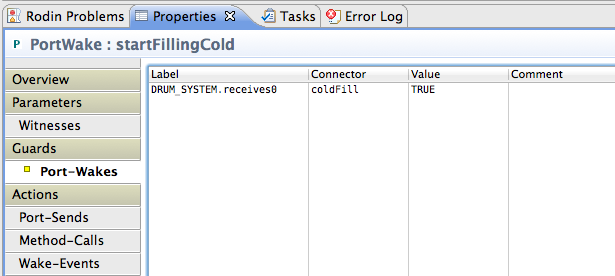
\includegraphics[width=1024]{figures/image45.png}
  \else
  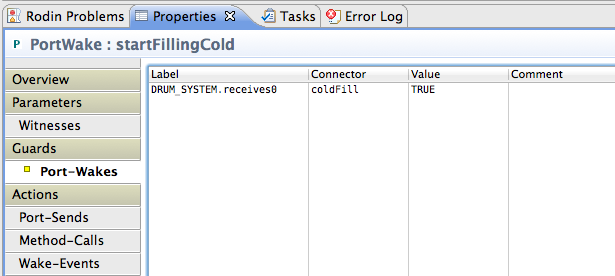
\includegraphics[width=1\textwidth]{figures/image45.png}
  \fi
  \caption{Fourth Refinement : Port Wake on the coldFill Connector}
  \label{fig:FourthRefinementPortWakeOnTheColdFillConnector}
\end{figure}  
 
The drum sub-system sends the value of water level and water temperature repeatedly at unit delay intervals using the self-wake operation sendLevel of Figure \ref{fig:FourthRefinementSelfWakeToRepeatedlySendOnLevelAndTempConnectors}.
 
 \begin{figure}[!htbp]
  \centering
  \ifplastex
  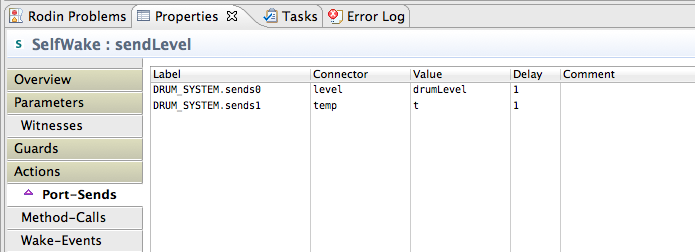
\includegraphics[width=1024]{figures/image46.png}
  \else
  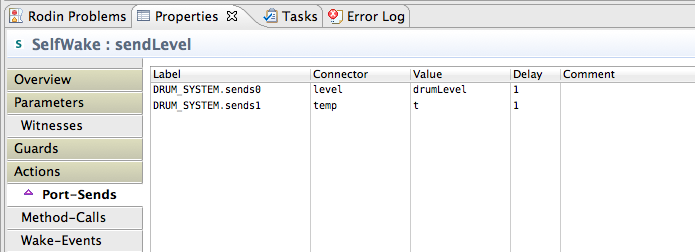
\includegraphics[width=1\textwidth]{figures/image46.png}
  \fi
  \caption{Fourth Refinement : Self Wake to Repeatedly Send on level and temp Connectors}
  \label{fig:FourthRefinementSelfWakeToRepeatedlySendOnLevelAndTempConnectors}
\end{figure} 
 
The washing machine sub-system switches off the water valve when it detects that the water level associated with the PID has been reached, as shown in Figure \ref{fig:FourthRefinementGuardedPortWakeToRespondWhenLevelReached}.
 
 \begin{figure}[!htbp]
  \centering
  \ifplastex
  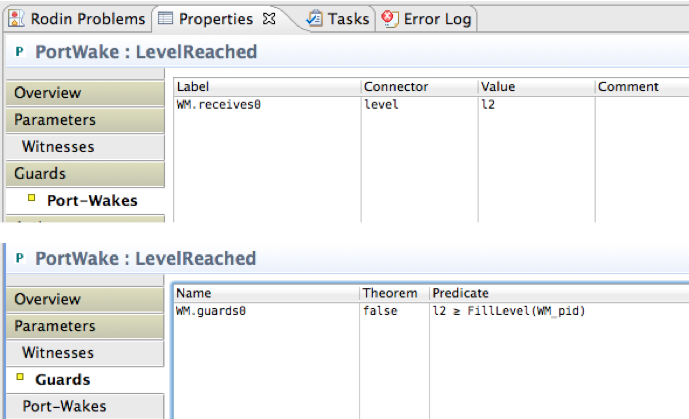
\includegraphics[width=1024]{figures/image47.png}
  \else
  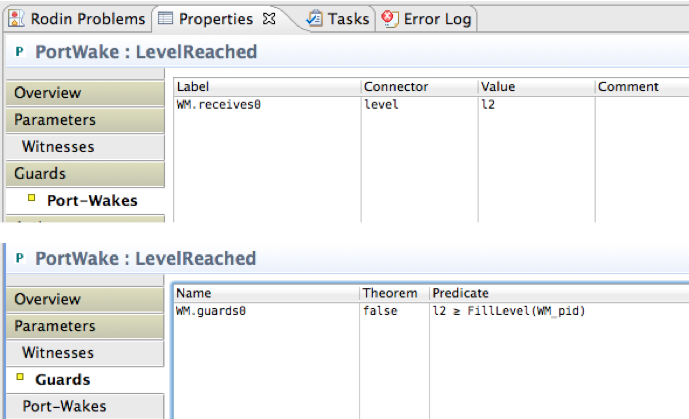
\includegraphics[width=1\textwidth]{figures/image47.png}
  \fi
  \caption{Fourth Refinement : Guarded Port Wake to Respond when Level Reached}
  \label{fig:FourthRefinementGuardedPortWakeToRespondWhenLevelReached}
\end{figure}  
 
The model checker is run again to show absence of deadlock. Note that because of the added complexity of this refinement, not all operations are covered (Figure \ref{fig:ProBModelCheckingCoverageForTheFourthRefinement}). Sufficient operations, however, have been covered to give confidence that filling operation is performing satisfactorily.
 
 \begin{figure}[!htbp]
  \centering
  \ifplastex
  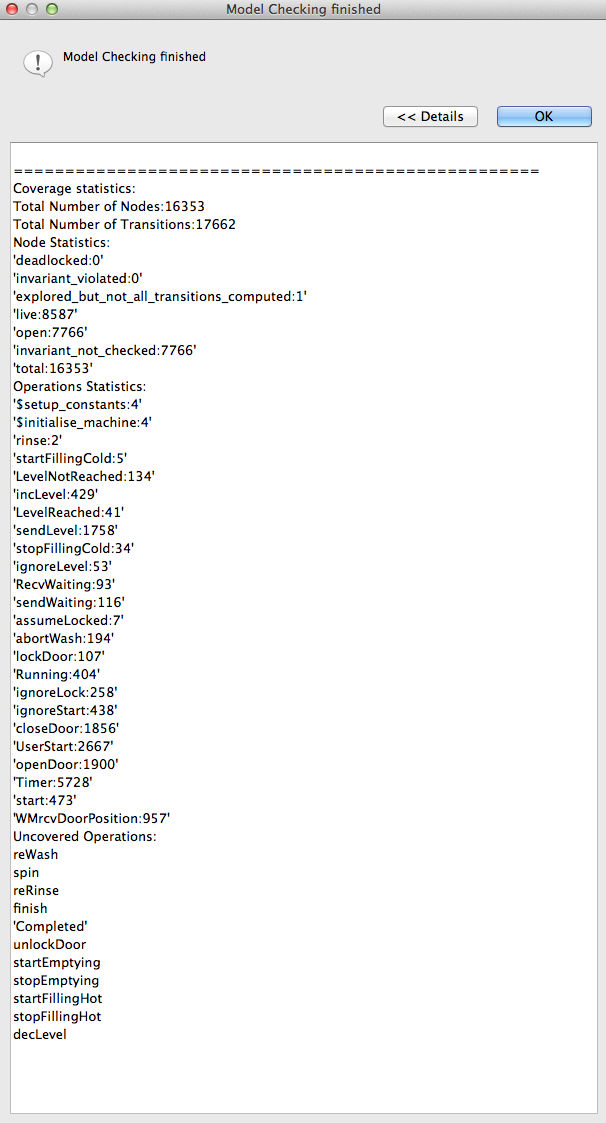
\includegraphics[width=1024]{figures/image48.png}
  \else
  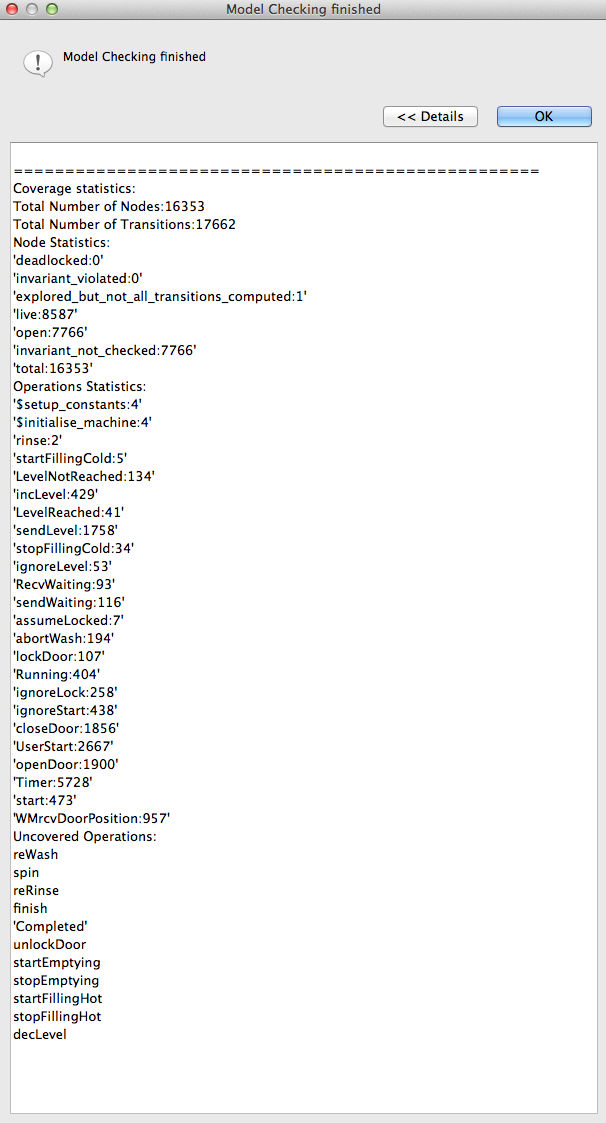
\includegraphics[width=1\textwidth]{figures/image48.png}
  \fi
  \caption{ProB Model Checking Coverage for the Fourth Refinement}
  \label{fig:ProBModelCheckingCoverageForTheFourthRefinement}
\end{figure}  


%%% Local Variables:
%%% mode: latex
%%% TeX-master: "component_diagrams-user_manual"
%%% End:
